\vspace{-2mm}
\section{Hybrid Programming Model}  \label{sec:programming_model}


\subsection{Hierarchical APIs}












\begin{figure}[t]
    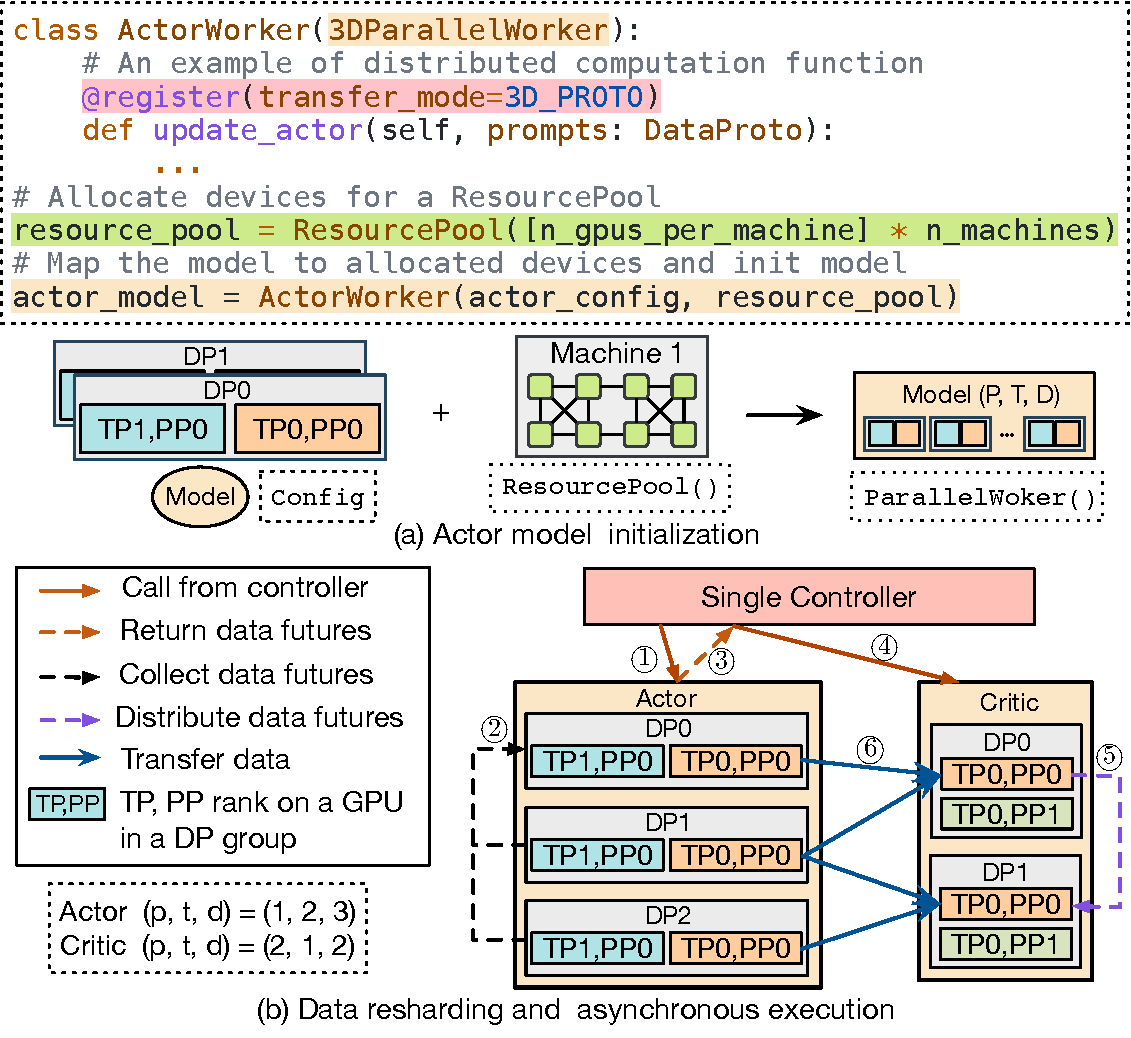
\includegraphics[width=\linewidth]{figs/fig_api_code_with_figures_highlight_box.pdf}
    \vspace{-8mm}
    \caption{An illustration of hierarchical APIs. (a) Model with 3D parallel configuration, resource allocation, and \texttt{3DParallelWorker} initialization. (b) Asynchronous data resharding between two models with collect and distribute functions in \texttt{3D\_PROTO}.
    }
    \label{fig:api_figure}
    \vspace{-5mm}
\end{figure}


\noindent\textbf{Intra-node: encapsulating distributed program.}
For distributed computation of each model
in different RLHF stages, we provide a base class, \verb|3DParallelWorker|. Given allocated devices, it facilitates distributed model weight initialization and establishes 3D parallel groups for each model. A parallel group includes a set of GPUs to host a specific parallel dimension of the model, e.g., different tensor shards in TP and different model replicas in DP. Figure~\ref{fig:api_figure}(a) illustrates initialization of the actor model with our APIs, while initialization of other models is similar.




Inheriting from the \verb|3DParallelWorker| class, several model classes, for actor, critic, reference, and reward model, respectively, are provided.
Each of these model classes encapsulates APIs to implement the model's distributed forward and backward computation, auto-regressive generation, and optimizer updates, decoupling the distributed computation code with data dependencies with other models.
These APIs can be easily implemented by reusing the computation scripts from existing LLM systems. For example, the computation involved in \verb|update_actor| function of \verb|ActorWorker| (the class for the actor model) is similar to the pre-training scripts in Megatron-LM~\cite{shoeybi2019megatron}. 
A model class encapsulates %
fundamental operations %
for implementing various RLHF algorithms, 
e.g., \verb|generate_sequences| in the actor model class for generating responses based on the prompts 
and \verb|compute_reward| in the reward model class for evaluating responses through a forward pass.
({More APIs are detailed in 
Appendix~\ref{appendix:primitive_apis}}).

Besides base class \verb|3DParallelWorker| that implements 3D parallelism, we further provide base classes for PyTorch FSDP (\verb|FSDPWorker|) and ZeRO (\verb|ZeROWorker|), and the corresponding model classes inheriting each base class, to support different parallelism strategies in model computation. ParallelWorker in Figure~\ref{fig:architecture} denotes one of these base classes.




\vspace{0.5mm}
\noindent\textbf{Inter-node: unifying data resharding implementation between models.} 
Many-to-many multicast is involved for data transfer between models employing different parallelism strategies on different devices. %
We unify this data transfer implementation
by associating each operation in each model class with a transfer protocol, using \verb|@register|. 
Each transfer protocol consists of a collect function and a distribute function, to aggregate output data 
 and distribute input data 
according to the parallelism strategy of each model. In the example in~\autoref{fig:api_figure}(a), \texttt{update\_actor} operation is 
{registered to}
transfer protocol \texttt{3D\_PROTO}, as 3D parallelism is used for actor training.
In \texttt{3D\_PROTO}, the collect function gathers all the {output data of corresponding model function (e.g., the loss scalar return from the \texttt{update\_actor})}
in each DP group to the single controller, and the distribute function distributes the input data {to the registered function (e.g., advantages for the \texttt{update\_actor})}
to each DP group. %
Data resharding is enabled using the source model's output collect function and the destination model's input distribute function. 
Figure~\ref{fig:api_figure}(b) illustrates data resharding between the actor (generation) and the critic (inference), where computation of the models adopts different 3D parallelism strategies.
The single controller gathers data futures using the collect function in \verb|3D_PROTO| of actor (steps $\textcircled{1}$-$\textcircled{3}$)  and sends it to 
critic (step $\textcircled{4}$); critic distributes the received data futures to each DP group using the distribute function in its \verb|3D_PROTO| (step $\textcircled{5}$).
Then %
remote data is retrieved from actor to critic, with each of critic's GPUs only fetching the required local batch of the actor's output data according to its DP rank (step $\textcircled{6}$). The actual data transfer only occurs between GPUs, avoiding any central bottleneck. 


We provide 8 transfer protocols, including \verb|3D_PROTO|, \verb|DP| \verb|_PROTO|, \verb|ONE_TO_ALL|, etc., that cover %
most data resharding scenarios 
({detailed in Appendix~\ref{appendix:transfer_protocols}}).
A user can further extend the transfer protocols %
through implementing customized collect and distribute functions.












\noindent\textbf{Facilitating flexible model placement.}
We provide a \verb|ResourcePool| class that virtualizes a set of GPU devices. 
When applying a \verb|ResourcePool| instance to a model class (Figure~\ref{fig:api_figure}(a)), distributed computation of the model will be mapped to the devices.
Models utilizing the same \verb|ResourcePool| instance are colocated on the same set of GPUs; %
models are placed on different sets of GPUs when different \verb|Resource| \verb|Pool| instances are applied in their model classes.
We assume no overlap between different \verb|ResourcePool| instances. 


\noindent\textbf{Asynchronous dataflow execution.}
When models are placed on separate sets of devices, their execution is triggered automatically %
as soon as their inputs become available~\cite {moritz2018ray}.
In Figure~\ref{fig:api_figure}(b), the data future from actor is immediately returned after the controller's call (steps $\textcircled{1}$-$\textcircled{3}$); the controller then initiates a new call to critic and distributes the futures following the %
transfer protocol (steps $\textcircled{4}$-$\textcircled{5}$). 
When some models are placed on the same set of devices, they are executed sequentially based on the calling order. %
With our programming model, \sysname{} is flexible in supporting diverse distributed execution patterns %
without any code change of the RLHF algorithm (Figure~\ref{fig:api_code}).











\begin{figure}[t]
    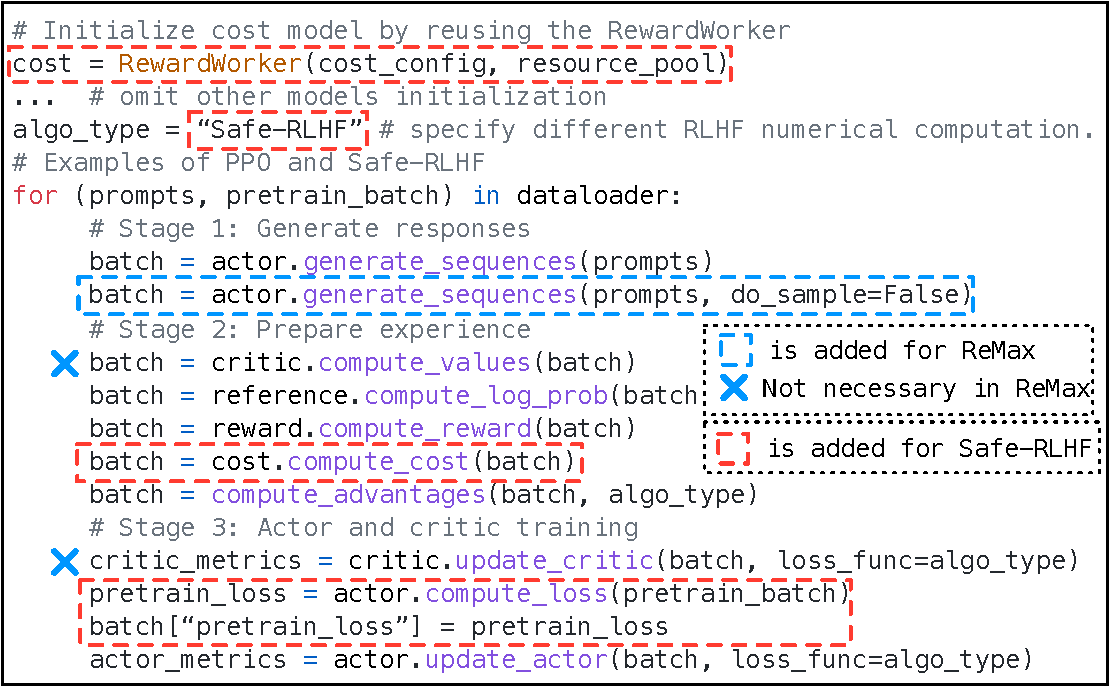
\includegraphics[width=\linewidth]{figs/fig_ppo_saferlhf_remax_test.pdf}
    \vspace{-7mm}
    \caption{Implementation of PPO~\cite{ouyang2022training}, ReMax~\cite{li2023remax}, and Safe-RLHF~\cite{daiSafeRLHFSafe2023}. Users can adapt to different RLHF algorithms by simply adding or deleting a few lines of code.}
    \label{fig:api_code}
    \vspace{-5mm}
\end{figure}

\subsection{%
Implementation of different RLHF algorithms} \label{sec:examples_of_RLHF_dataflow}

Our APIs %
enable streamlined development of various RLHF algorithms (dataflows). 
Users can implement an RLHF algorithm in a few lines of code as a single process program to run on the single controller,
that involves a sequence of primitive API calls to invoke distributed computation of models. 
Examples of PPO, ReMax, and Safe-RLHF are given in Figure~\ref{fig:api_code}. PPO can be implemented in just 8 lines by invoking model operations
including \texttt{compute\_values} and \texttt{generate\_sequences}, which are executed under the multi-controller paradigm on multiple GPUs.
To adapt to Safe-RLHF which integrates an additional cost model to evaluate safety preferences and %
the pre-taining loss for actor, only 5 more lines of code are added on top of PPO implementation.
{To adapt to ReMax, one additional call to actor generation is needed, and the critic-related code can be removed.}

\noindent \textbf{Achieving flexible.}
This flexibility of extension is crucial for researchers to explore different RLHF algorithms: they can reuse distributed computation encapsulated in each model class and 
simply adjust the code for numerical computations according to specific algorithms, such as GAE~\cite{schulman2018highdimensional} and KL divergence in \verb|compute_advantage| and loss functions of actor and critic.
The streamlined development can be attributed to %
the hybrid programming model.
Our modular API design simplifies development, facilitates extensive code reuse, %
and enables directly incorporating the codebase of existing LLM training/serving frameworks. 
It also decouples model computation and data transfer among models. 
Any change in the distributed frameworks does not affect the code of the RLHF algorithm (Figure~\ref{fig:api_code}), enabling individualized optimization for each model's execution (\textsection\ref{sec:hybrid_engine}).
Flexible placement of models with diverse workloads is supported, %
enabling optimized mapping of RLHF dataflow onto various devices (\textsection\ref{sec:auto_mapping}).









